\cleartooddpage[\thispagestyle{empty}]
\newcommand{\EReco}{$\textrm{E}_{\textrm{Reconstructed}}$}
\newcommand{\ETrue}{$\textrm{E}_{\textrm{True}}$}

\chapter{Gamma-Ray Reconstruction Methods}\label{ch:grrecon}

Chapter \ref{chapter:veritas} explained how the trigger system initializes the readout of PMT voltage traces.
This chapter describes how gamma rays are reconstructed.
In gamma-ray reconstruction, voltage traces induced by Cherenkov photons must be identified and combined to form an image of the original Cherenkov shower.
Then the shower images from multiple telescopes can be used to reconstruct the original gamma ray's energy and direction.

Throughout the rest of this thesis, \textit{Galactic Center} and \textit{Sgr A*} are used to describe the main analysis region.
While in astrophysics \textit{Galactic Center} refers to the several-degree-radius area around the center of our galaxy, \textit{Sgr A*} refers to the specific central gamma-ray point source (<\ang{0.2} radius).
VERITAS data observations that cover this point source are also referred to as \textit{Sgr A*} data, described further in Section~\ref{veritasdata}.


\section{Pedestal Variation}
Before reconstructing any events, the pedestal and pedestal variations must be calculated.
This is done by artificially triggering all pixels once per second during observations, in order to record events that contain only noise.
The \textit{pedestal} is the average of the digital counts (dc) of all noise events for each pixel.
From this pedestal, the pedestal variations are then calculated for each pixel as the root mean square of all the dc counts in all noise events.
In this context, noise events can be due to night-sky-background photons, or from electronic noise.

\section{Pixel Identification}
The first step to reconstruct events is to determine which pixels are part of a shower image.
This is done by subtracting the dc pedestal from the entire trace, and then summing all trace bins within a fixed window, called the integration length, to get the total dc.

Most voltage traces have the same general shape: a quickly rising start of the pulse, followed by a longer, slowly falling tail.
This can be seen in Figure~\ref{fig:pmt_pulse_widths} in the previous chapter.
To act as a point of reference in each voltage pulse, the time when the voltage trace is at half of its maximum value is called $T_{0}$.
The trace is then integrated a second time using a smaller 14- or 24-ns-wide time window, starting at $T_0 - 30\%$, to reduce the inclusion of dc from NSB photons and electronic noise.
This integration is the first of two passes, usually referred to as the double-pass method~\cite{doublepass}.
If a pixel's first-pass total dc is higher than 5 times the pedestal variation, then it is classified as an image pixel.
If it is between 2.5 and 5 times the pedestal variation, it is considered a border pixel.

Once all pixels have been classified, isolated border pixels that have no neighboring image pixel are removed from the image, as they are more likely to be due to noise than Cherenkov photons.
Then, the time gradient from the image and border pixels can be found by performing a linear fit of the $T_{0}$ times.
This time gradient can then be used to place a third integration window 
with 30\% of the window before each pixel's $T_{0}$, to more accurately measure the charge due to Cherenkov photons in the pixel.
This third integration window is the second pass in the double-pass method.

From the image pixels, border pixels, and charge in each pixel, the shower's Hillas parameters~\cite{hillas_params} can be calculated.
These parameters include the shower size in photoelectrons (or equivalent units), center of charge, angle, length, and width.
The center of charge is the charge-weighted average of all image and border pixel positions.
The angle of the shower determines how the image's major axis is oriented in the camera.
The shower length and width are determined by the root mean square of the shower image along its major and minor axes, respectively, as shown in Figure~\ref{fig:shower_param}.
  
\begin{figure}[t]
  \centering
  \includegraphics[width=0.45\textwidth]{images/shower_parameter_diagram/diagram.pdf}
  \caption[Basic Shower Diagram]{
    An example shower image in one VERITAS camera.
    The gray circles are the locations of PMTs.
    Red circles are PMTs that have detected Cherenkov photons.
  }
  \label{fig:shower_param}
\end{figure}
\FloatBarrier

\section{Position Reconstruction}\label{subsec:posrecon}
By examining the images from multiple telescopes, the initial direction of the event can be determined.
This is done by overlapping all telescope images in a single sky coordinate system, and projecting each image's major axis backward in time.
These axes should intersect very close together, and the average of the intersection points determines the event's initial direction.
The axes tend to not intersect perfectly due to the finite resolution of the camera pixels.
Additionally, night sky background photons and atmospheric absorption can add and remove photons from the shower image.

When averaging the intersection points, weights can be applied to each intersection based on the angle between the two lines.
This improves the reconstruction, because the intersection point from two images at \ang{90} angles will be less sensitive to image fluctuations than two images at \ang{160}, as shown in Figure~\ref{fig:largeintersectangle}.
Additionally, the \textit{disp} method is explored in Section~\ref{subsec:disp} to provide improvements at lower telescope elevations.
This would be beneficial as the Galactic Center is at a low (<\ang{50}) telescope elevation (see Figure~\ref{fig:datapointingelevations}).

\begin{figure}[!t]
  \centering
  \includegraphics[width=0.95\textwidth]{images/large_angle_image_intersection_error/laiie_cropped.pdf}
  \caption[Large Image Intersection Angles]{
    In diagram (a), when a noisy pixel is added to an image, the reconstructed position is only moved a small distance (the orange arrow).
    In diagram (b), due to the large angle between images, the error in the reconstructed position is much larger.
  }
  \label{fig:largeintersectangle}
\end{figure}
\FloatBarrier

\subsection{Angular Reconstruction with Boosted Decision Trees}\label{subsec:disp}
At high elevations, shower images often form small intersection angles, because the telescopes are spread out in two dimensions, relative to the shower in the atmosphere.
At low elevations near the Galactic Center, however, the telescope array flattens into one dimension, which makes the shower's impact parameter (the shortest distance between the telescope and the shower core axis) smaller for two of the telescopes.
These two closer telescopes then have very short, almost circular images, which makes them more sensitive to noisy pixels or shower fluctuations, as shown in Figure~\ref{fig:showerhighlowelev}.
This also causes the remaining telescope images to have large intersection angles, which also reduces the accuracy of the position reconstruction.

\begin{figure}[!t]
  \centering
  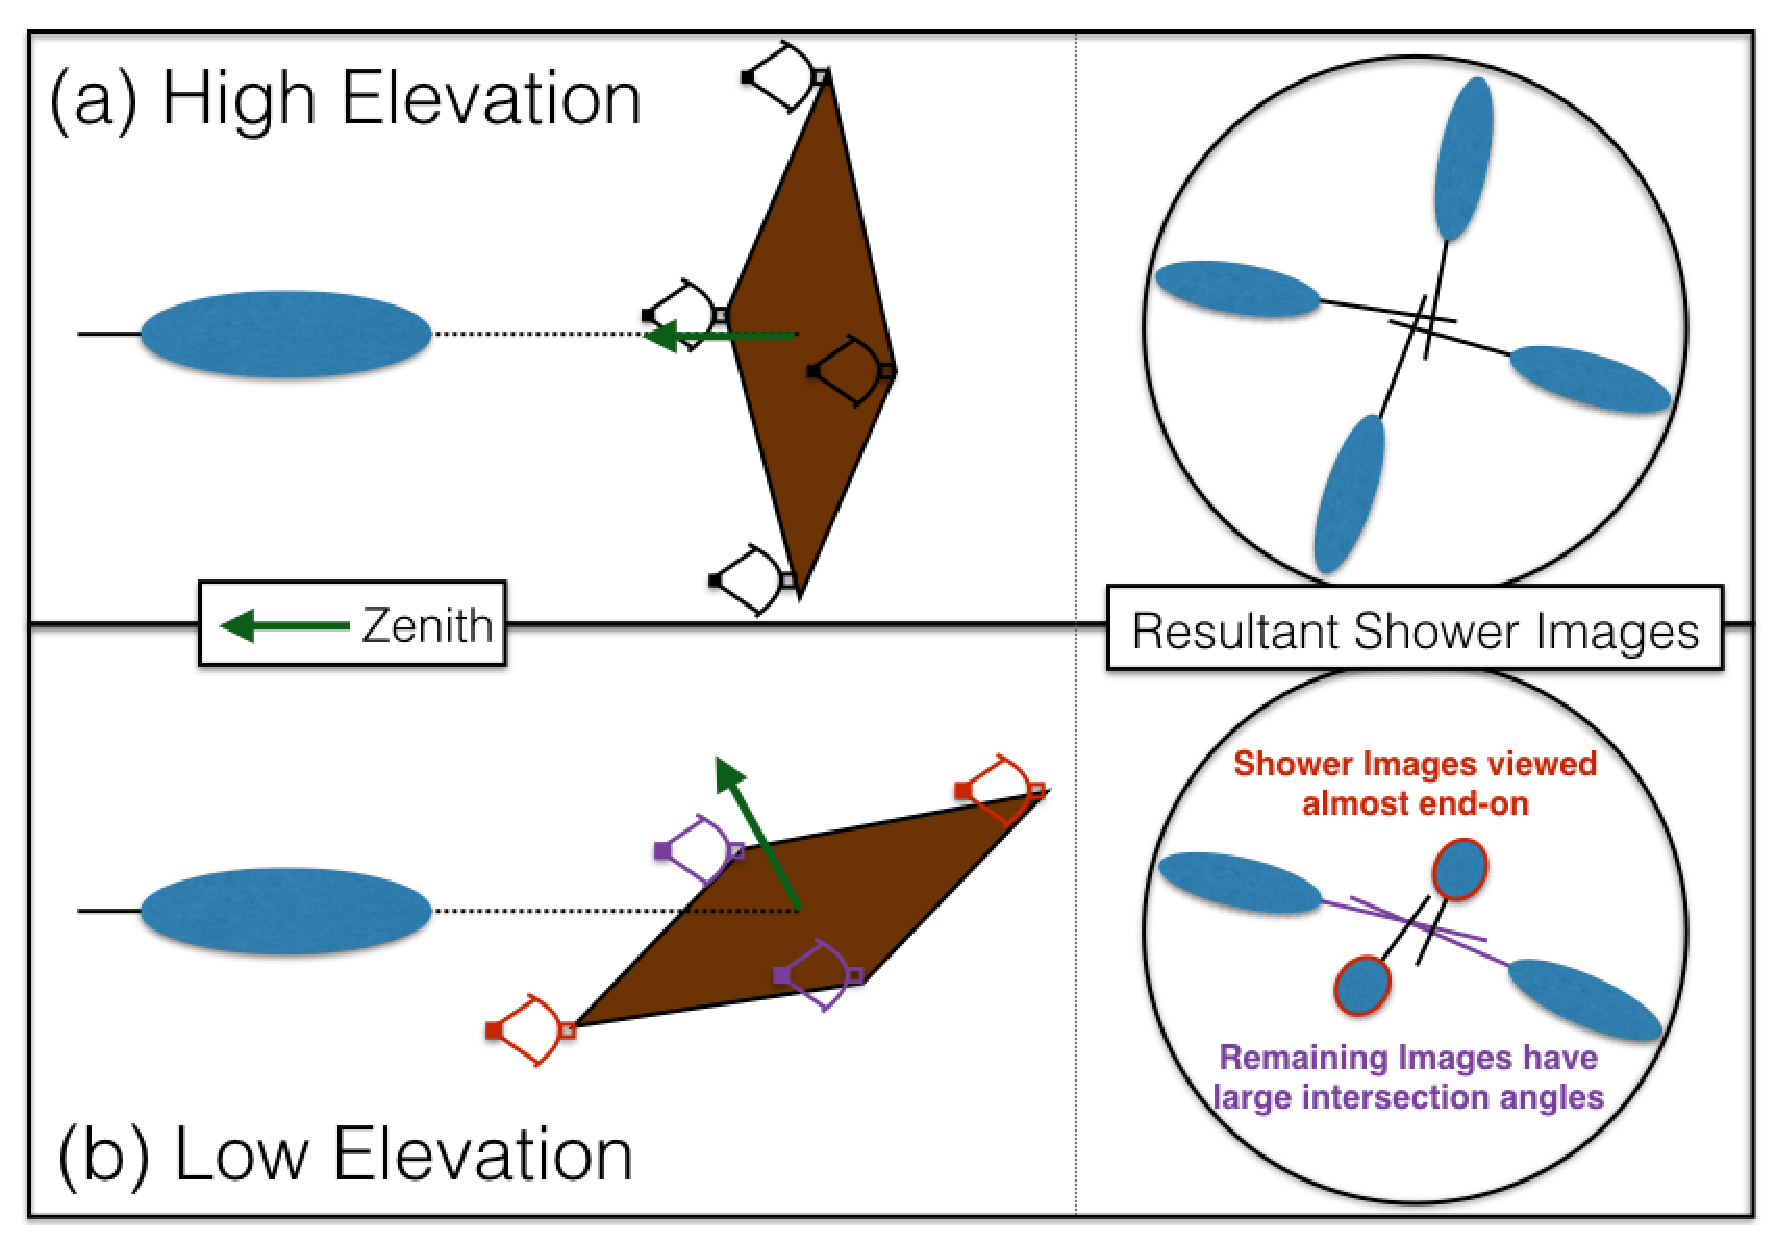
\includegraphics[width=0.55\textwidth]{images/high_elevation_vs_low_shower_images_cropped.eps}
  \caption[Shower Images at High and Low Elevations]{
    In Figure (a), high elevation showers produce long images in all four telescopes.
    In Figure (b), lower elevation showers produce shortened images in two telescopes, and the remaining images form large angle intersection.
  }
  \label{fig:showerhighlowelev}
\end{figure}

To better handle these near-parallel image axes at low elevations, the reconstructed position can be determined from more parameters than just the weighted image axes intersection points.
From simulations, the distance between the center of the Hillas shower image and the true position can be calculated, where the angular distance between the two is the disp parameter~\cite{Senturk:2011}, shown in Figure~\ref{fig:dispdiagram}.
Then, this disp parameter can be provided to a machine learning algorithm~\cite{Beilicke2012NIM}, along with other image parameters like:
\begin{quote}
  \begin{description}[noitemsep]
    \item [width:] image angular width;
    \item [length:] image angular length;
    \item [wol:] $\frac{\textrm{width}}{\textrm{length}}$;
    \item [size:] total image dc;
    \item [ntubes:] number of pixels in the image;
    \item [loss:] fraction of image pixels at the edge of the camera;
    \item [asym:] distance between image center-of-dc and the pixel with the highest dc;
    \item [tgrad:] the slope of the linear time fit to the pixel arrival times;
    \item [cross:] angular distance between the image center and the average intersection point of the image axes.
  \end{description}
\end{quote}
% list of training parameters: grep "AddVariable" $EVNDISPSYS/src/trainTMVAforAngularReconstruction.cpp
% how variables are calculated: grep -P "fParGeo.+\=" $EVNDISPSYS/src/VImageParameterCalculation.cpp
% asym: http://inspirehep.net/record/1395717/files/RdelosReyes.pdf
% Once trained on these parameters, the machine learning algorithm can construct a boosted decision tree for determining any new image's \textit{disp}, which can then be used with the image axes intersections to improve the gamma-ray reconstructed positions.


\begin{figure}[t]
  \centering
  \includegraphics[width=0.4\textwidth]{images/disp_parameter/disp_parameter.pdf}
  \caption[Angular Reconstruction Disp]{
    The disp parameter is the angular distance between the center (red dot) of a Hillas image (blue oval) and the true sky position (green dot).
    Generally, longer shower images have a larger disp angle.
  }
  \label{fig:dispdiagram}
\end{figure}

% https://veritas.sao.arizona.edu/wiki/index.php/BDT_Angular_reconstruction
These parameters for 17,000 simulated showers were used to train boosted decision trees (BDTs) that estimate the disp for a new shower's images.
This estimated disp can then be combined with the image axes intersection points to more accurately reconstruct the original gamma-ray point of origin.

Once the training is complete, it is tested on a separate set of 17,000 simulated events, whose true and predicted disps plotted in Figure~\ref{fig:disptraining}.
The x-axis describes the true disp value for each event, while the y-axis describes the disp value estimated by the BDT, with a black $x=y$ line marked, which represents a perfect 1:1 disp reconstruction.
To examine how close the predicted disp is to the true disp, a residual plot is shown in Figure~\ref{fig:dispresidual}.
It shows the $\frac{\textrm{Predicted disp}}{\textrm{True disp}}$ for each true disp bin, including $\pm$ 1 standard deviation error bars.
From this residual plot, it can be seen that in nearly all bins the predicted disp is consistent with the true disp.

% made from screenshot of last slide in Dropbox/Presentations/20160719_Group_Meeting.key
\begin{figure}[b]
  \centering
  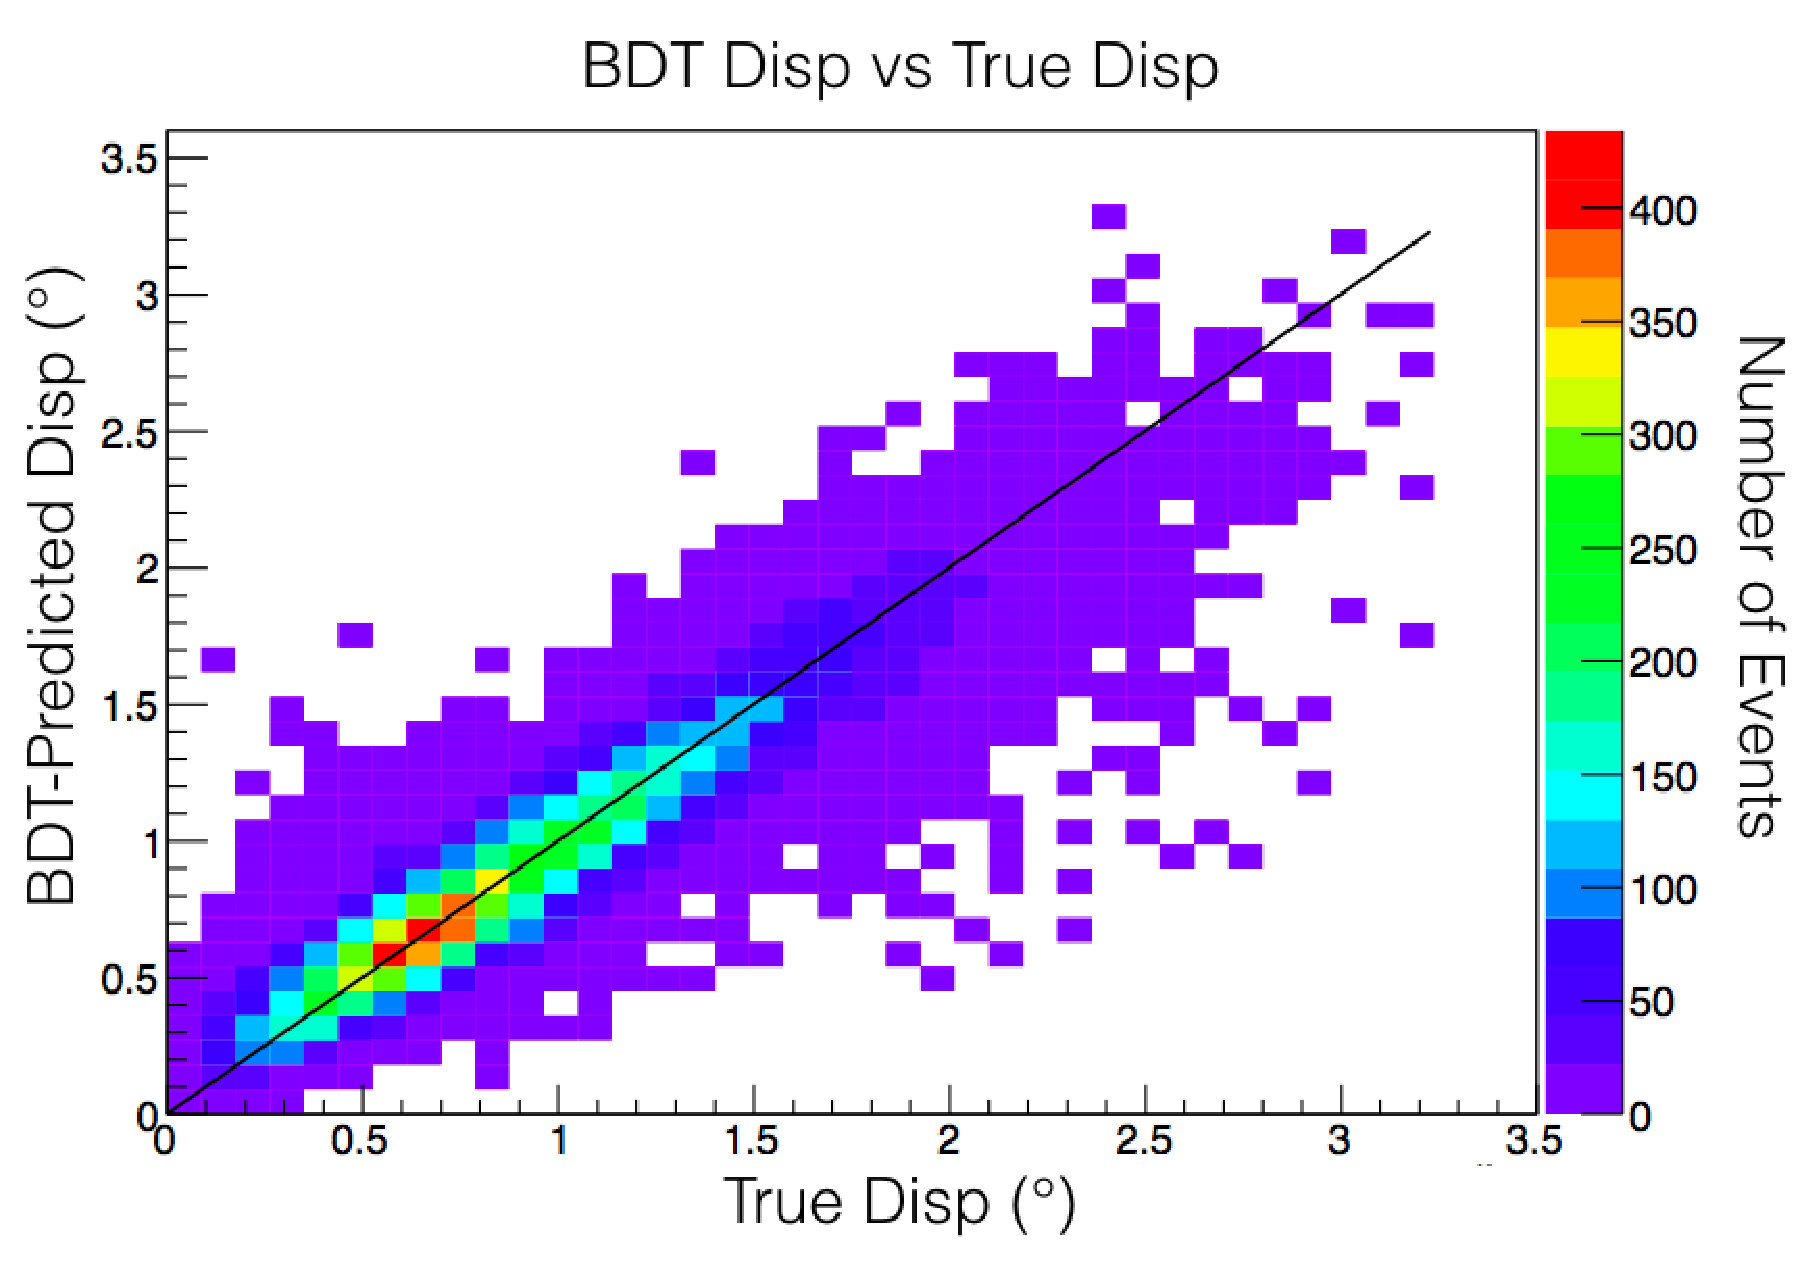
\includegraphics[width=0.85\textwidth]{images/disp_training/disp_training.eps}
  \caption[Disp BDT Training]{
    The true disp vs the BDT-predicted disp, for \nicetilde17,000 gamma-ray event images in T1, from \SI{500}{\GeV{}} to \SI{200}{\TeV{}}.
  }
  \label{fig:disptraining}
\end{figure}

\begin{figure}[t]
  \centering
  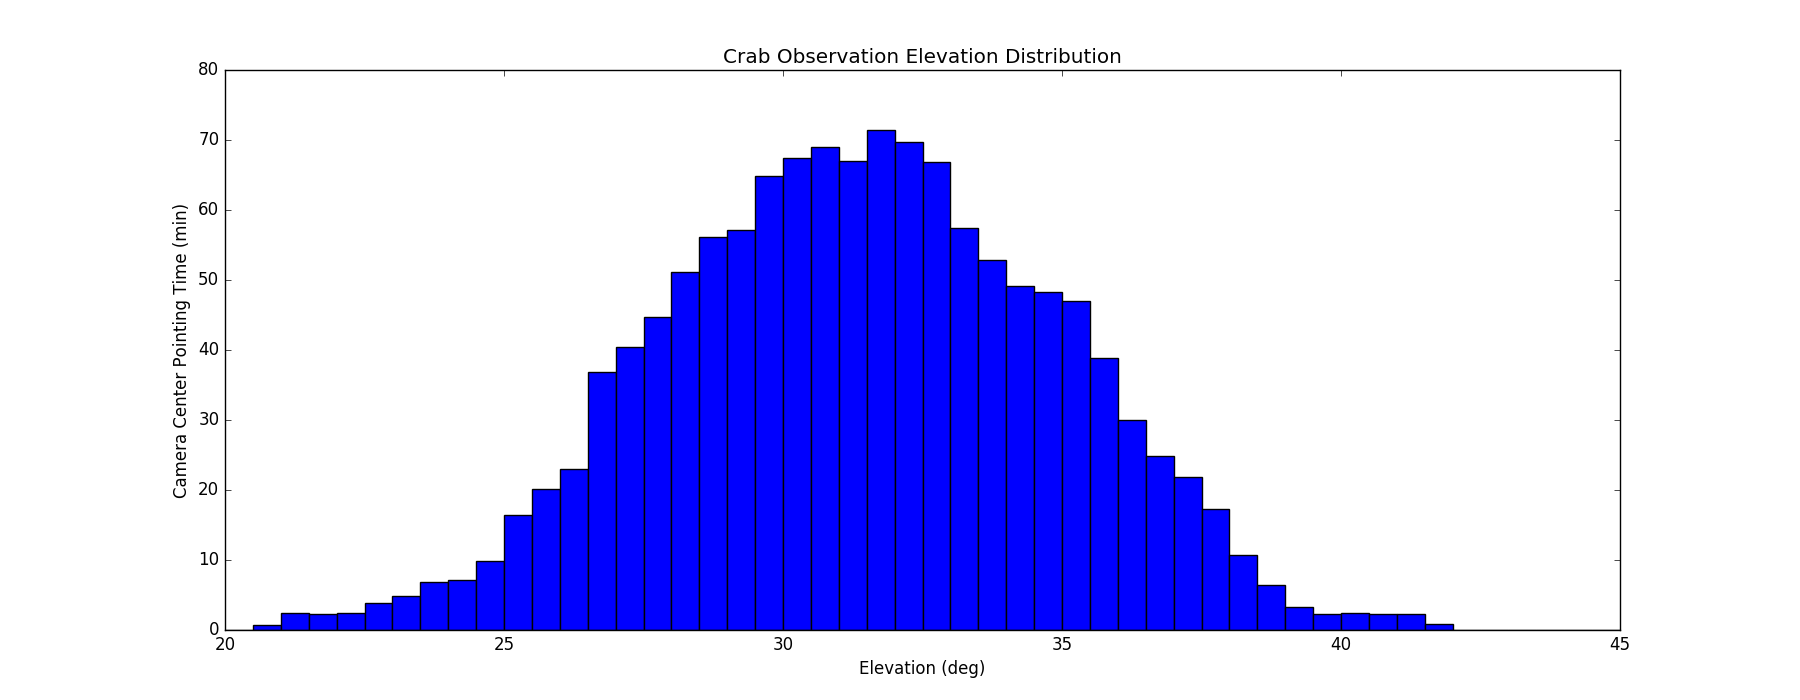
\includegraphics[width=0.85\textwidth]{images/disp_training/improved_disp_plot/plot.pdf}
  \caption[Disp BDT Residual]{
    The predicted/true disp residual, from the bins in Figure~\ref{fig:disptraining}.
    The error bars represent 1 standard deviation.
    The graph is split at $x=0.75^{\circ}$ to keep the error bars visible.
  }
  \label{fig:dispresidual}
\end{figure}

To examine the effect this disp method has on an analysis, the point spread functions (PSFs) are compared.
The PSF describes how much a group of events from the same point source are spread out due to being imperfectly reconstructed.
In general, PSFs are quantified by their 68\% containment radius, the angular radius around a point source which contains 68\% of the reconstructed events.
PSFs are discussed further in Section~\ref{subsec:psf}.
The PSF containment radius is calculated from simulations, with both the disp reconstruction method and the regular geometric reconstruction method.
The ratio of the $\frac{\textrm{disp PSF radius}}{\textrm{geometric PSF radius}}$ is shown in Figure~\ref{fig:disp_psf_comparison}.
Because the PSF changes with telescope elevation, telescope azimuth and zenith, night sky background noise, atmosphere, and offset from the camera center, the average PSF at each gamma-ray energy is shown.
This PSF is the average over the two data sets used in this analysis, the Crab Nebula and the Galactic Center, described further in Chapter~\ref{chapter:analysis}.
The average PSF for the Crab Nebula data is shown by a green line and a green 1-standard-deviation error band, and similarly the Galactic Center is shown in blue.
    
Figure~\ref{fig:disp_psf_comparison} shows the disp method does offer a minor improvement at low energies, but is worse at higher energies, though both are within the statistical uncertainties.
The lack of improvement may be due to the use of boosted decision trees that were not optimized for this particular analysis.
%, whereas a previous study with this method utilized a lookup table of six parameters, described in Ref.~\cite{Beilicke2012NIM}.
Nevertheless, the analysis described in Chapter~\ref{chapter:analysis} utilizes the disp method when reconstructing gamma-ray events.
    
\begin{figure}[b]
  \centering
  \includegraphics[width=0.95\textwidth]{images/disp_event_offset_hists/plot_offset0_50.pdf}
  \caption[DISP Point Spread Function Comparison]{
    Comparison between the disp and geometric point spread function 68\% containment radii.
    The lines represent the average ratio, with a 1 standard deviation error band.
    Green is from the Crab Nebula data, and blue is from the Galactic Center data.
    The average PSF shown is at a \ang{0.5} offset from the camera center.
  }
  \label{fig:disp_psf_comparison}
\end{figure}

\FloatBarrier

\section{Energy Reconstruction}\label{subsec:enrecon}

To reconstruct the energy of each shower, a lookup table of simulated showers is assembled.
This database stores the median energy of the showers, as well as the spread of the distribution of shower energies.
However, a shower's energy is strongly correlated with two measured parameters.
The first is the shower's \textit{image size}, the number of observed Cherenkov photons.
The second is the \textit{core distance}, the distance between the VERITAS array center and where the central shower axis intersects the ground.
Showers are therefore divided into subgroups based on this size and distance, then the median energy and energy spread of each subgroup are stored in the lookup table.

The medians and spreads also vary based on the telescope, noise level, telescope azimuth and zenith angle, offset from camera center, and epoch, so additional showers are simulated at a variety of these parameters, and added to the lookup table.
If any of these parameter space points were partially or completely combined, they would result in a larger error on the reconstructed energy.

One point in the parameter space of this lookup table is shown in Figure~\ref{fig:energy_params}.
In the left plot, the median energy is shown at at several shower core distances and image sizes.
In the right plot, the spread in the energy distribution is shown at the same distances and sizes.
By looking up a shower's size and distance in this table, the shower's true energy can be reconstructed.

\begin{figure}[bh]
  \centering
  \includegraphics[width=\textwidth]{images/energy_table_plots/energy.pdf} &
  \caption[Energy Table Parameters]{
    The median shower energy, and spread in energy, for several image sizes and core distances.
    The median shower energy is shown in the left plot, the right plot shows the $2\sigma$ spread in energy at the same parameter space points.
  }
  \label{fig:energy_params}
\end{figure}

Once an energy has been estimated for each telescope's shower image, they are combined with the weighted average in Equation~\ref{eqn:en_avg}, where $E_i$ is the $i^{\textrm{th}}$ telescope's energy and $\sigma_x$ is the $x^{\textrm{th}}$ telescopes energy distribution.

\begin{equation}\label{eqn:en_avg}
  E = \frac{ \sum_{i=1}^{N} \frac{E_i}{ \sigma_{i}^2} }{ \sum_{j=1}^N \frac{1}{ \sigma_{j}^2 } }
\end{equation}


\section{Gamma-Hadron Separation}

After characterizing the direction and energy of each shower, the next step is to remove the considerable fraction (\nicetilde1000:1) of showers that were induced by protons.
This process is often referred to as Gamma-Hadron separation.
When the lookup table in Section~\ref{subsec:enrecon} is constructed, the medians and spreads of the showers' lengths and widths are stored alongside the energies.
The length and width of one shower image are described in Figure~\ref{fig:shower_param}.
A group of these median widths are shown in Figure~\ref{fig:mscw_params}.
These show how the shower width varies with core distance and image size.

\begin{figure}[b]
  \centering
  \includegraphics[width=0.5\textwidth]{images/mscw_table_plots/mscw.pdf} &
  \caption[Shower Median Width]{
    Plots of the shower widths from the lookup table.
    The median shower width is shown at several shower core distances and image sizes.
  }
  \label{fig:mscw_params}
\end{figure}

These stored lengths and widths can then be used to create new parameters \textit{mean reduced scaled length} (MRSL) and \textit{mean reduced scaled width} (MRSW), calculated with Equation~\ref{eqn:mscwl}~\cite{mrswl_technique}.

\begin{equation}\label{eqn:mscwl}
  \begin{split}
    \textrm{MRSL}_{\textrm{shower}} & = \frac{1}{N_{\textrm{images}}} \sum_{i}^{N_{\textrm{images}}} \frac{l_{i}-l_{\textrm{median}}}{l_{\textrm{spread}}} \\
    \textrm{MRSW}_{\textrm{shower}} & = \frac{1}{N_{\textrm{images}}} \sum_{i}^{N_{\textrm{images}}} \frac{w_{i}-w_{\textrm{median}}}{w_{\textrm{spread}}} \\
  \end{split}
\end{equation}

In this equation, $l_{\textrm{image}}$ and $w_{\textrm{image}}$ are each observed image's length and width.
Multiple images of the same shower can be combined to calculate the $MRSL_{\textrm{shower}}$ and $MRSW_{\textrm{shower}}$ for each shower.
The parameters $l_{\textrm{median}}$ and $w_{\textrm{median}}$ are the median length and width from the lookup table.
The parameters $l_{\textrm{spread}}$ and $w_{\textrm{spread}}$ are the spread in length and width distributions, also from the lookup table.
The parameter $N_{\textrm{images}}$ is the number of triggered telescope images.
Gamma-ray showers and proton showers have different distributions of MRSL and MRSW (proton showers tend to be wider at a given length), so cuts can be applied based these two parameters to partially filter out the proton showers.

These two distributions can be seen in Figure~\ref{fig:mscw_crab}.
In it, the MRSWs of events near the Crab Nebula are shown as a green histogram.
The red histogram shows the MRSWs of events in several nearby regions which don't have any sources of gamma rays.
The red histogram events are weighted by the number of off regions, so that both red and green distributions are scaled to the area of a single region.
These off regions are the same size as the on region, and are radially-symmetric around the camera center.
The excess of green events between $-2<\mathrm{MRSW}<0$ are the gamma-ray-like events from the Crab Nebula.
The on region shows a slight peak that is not quite centered at $\mathrm{MRSW}=0$, likely due to using simulations that were not tuned for these low elevations (see Section~\ref{veritasdata}).
See Ref.~\cite{Krause2017} for a more thorough discussion on gamma-hadron separation.

\begin{figure}[th]
  \centering
  \includegraphics[width=0.8\textwidth]{images/mscw_table_plots/mrsw_crab.pdf} &
  \caption[Crab Nebula Mean Reduced Scaled Width]{
    Plots of the MRSWs for events in the Crab Nebula analysis described further in Section~\ref{sec:crab_analysis}.
    The green histogram is the MRSWs for events within \ang{0.25} of the Crab Nebula, and should contain many gamma-ray events with a smaller MRSW.
    The red histogram is the MRSWs for events in several off regions, which should only contain proton-induced showers, which will have larger MRSWs, as proton showers tend to be wider than gamma-ray showers.
  }
  \label{fig:mscw_crab}
\end{figure}


\section{FITS Conversion for GammaLib and ctools}\label{fitsconversion}
Once gamma rays have been reconstructed with Eventdisplay, they must be exported to GammaLib and CTOOLS~\cite{gammalibctools}.
GammaLib and CTOOLS are software that perform the likelihood calculation, which is described further in Section~\ref{sec:likeratio}.
This software possesses several useful features, including automatic model convolution with instrument response functions (IRFs) and easier comparison with results from other gamma-ray telescopes like H.E.S.S. and MAGIC.
This software is also one of the main high-level analysis tools to be used by the Cherenkov Telescope Array (CTA), making it and easier to include VERITAS data into future CTA analyses.

Exporting gamma-ray data to this software involves converting the event list and IRFs to a FITS file format.
The IRFs consist of the effective areas, the point spread functions, the background models, and the energy dispersion, defined in Sections~\ref{subsec:effarea}-\ref{subsec:edisp}.
%The effective area quantifies the total gamma-ray collection area of the observatory, which is needed for spectral measurements.
%The point spread function quantifies the distribution of reconstructed positions for a given true position, which is needed for modeling point sources and extended spatial structures.
%The background models measure the relative number of observed events in different parts of the camera.
%The energy dispersion quantifies the distribution of reconstructed energies for a given true energy.
During the export, several decisions are baked into the event lists and IRFs.
As this thesis revolves around an analysis at an elevation of \nicetilde{}\ang{30}, the IRFs may rapidly change with time.
At this elevation, with VERITAS's field of view of \ang{3.5}, the air mass column density ($\textrm{g}/\textrm{cm}^2$) is 12\% higher at the bottom of the camera than at the top.
% see veripy.atmo_column_density() for 12% calculation
Combined with the fact that an observing target can move several degrees over one \SI{30}{min} observation, this means the air mass can change by several percent over a single 30-minute observation.
This changing atmosphere would mean the IRFs at the beginning of an observation may be measurably different than at the end of an observation.

To reduce the impact of this, observations are broken up into 8-minute-long parts.
For each of these 8 minute parts, IRFs are exported alongside the observation.
A part's average elevation, azimuth, and night sky background rate are used to select the best-matching IRFs for that part.

The next subsections discuss each IRF individually.
The effective areas are described in Section~\ref{subsec:effarea}, the point spread function in Section~\ref{subsec:psf}, the background models in Section~\ref{background_production}, and the energy dispersion in Section~\ref{subsec:edisp}.

\FloatBarrier
  
\subsection{Effective Area}\label{subsec:effarea}
% use effective area as a casual noun!
% plot of effective area vs energy
Effective area is the measure of how large an observatory's collection area is, which determines how many gamma rays can be detected per unit time, solid angle, and energy.
The effective areas are calculated with \nicetilde 25 million Monte Carlo gamma-ray shower simulations for each point in the atmosphere/elevation/noise/offset parameter space.
These simulations are created using the CORSIKA package~\cite{corsika1998}.
% where $VERITAS_USER_DATA_DIR = /lustre/fs19/group/cta/users/nkelhos/VERITAS/
% see $VERITAS_USER_DATA_DIR/figure_out_number_of_simulated_showers/read.py
% run read.py, number of packets is roughly the number of showers, after core 
% rescattering and offset wobbling for one point in the parameter space
% # of points:
%   10 elevations
%    2 atmospheres
%    9 wobbles
%    9 noises (care only, grisu doesn't simulate noise)
This is done in the shower plane, the plane perpendicular to the line drawn between a pointing target and the center of the observatory.
The effective area is then calculated via:
$A=\pi R^2 \frac{N_{\text{survived}}}{N_{\text{simulated}}}$
where R is the radius of the area within which simulated showers are directed to fall, $N_{\text{simulated}}$ is the number of showers that were initially simulated into the area, and $N_{\text{survived}}$ is the number of simulated showers that pass all cuts.
This effective area is thus a measure of how much detection area the observatory would have if it had a 100\% detection efficiency, which can then be used in calculating a source's flux.
Figure~\ref{fig:effarea_paramspace} shows how the effective area peaks at \nicetilde{}\SI{3e5}{m${}^2$} for \SI{3}{\TeV{}} events at the camera center.

\begin{figure}[!t]
  \centering
  \includegraphics[width=0.85\textwidth]{images/effarea_plots/effarea_space.pdf}
  \caption[Effective Area Parameter Space]{
    Effective areas at different points in the energy and camera offset parameter space for run 78128.
    Data is shown as the black points, indicating the position of some events from that run in the parameter space.
    The color axis indicates the effective area, calculated from simulations, at different gamma-ray energies and distances from the camera center.
  }
  \label{fig:effarea_paramspace}
\end{figure}

For the the Crab Nebula and Sgr A* data, the effective areas of all events are shown in Figure~\ref{fig:effarea_usage}.
The Crab Nebula acts as a known \textit{standard candle} source to test out the analysis, before attempting to search for dark matter within the Sgr A* data.
    
    \begin{figure}[!t]
      \centering
      \begin{tabular}{c}
        \includegraphics[width=0.85\textwidth]{images/effarea_plots/effarea_events_crab.pdf} \\
        \includegraphics[width=0.85\textwidth]{images/effarea_plots/effarea_events_sgra.pdf}
      \end{tabular}
      \caption[Effective Areas Used]{
      The effective areas used by all events in each analysis.
      From these plots, it is easy to check for events with anomalously high (>\SI{400000}{m${}^2$}) or low (\nicetilde\SI{0}{m${}^2$}) effective areas.
      }
      \label{fig:effarea_usage}
    \end{figure}
  
  \FloatBarrier

  \subsection{Point Spread Function}\label{subsec:psf}

    When reconstructing the source position of each gamma ray, it is necessary to know the uncertainty of the position.
    Errors in the position primarily come from the randomness of shower images.
    The same gamma ray may be reconstructed to have different energies or come from different directions, due to the following:
    
    \begin{itemize}[label=$\bullet$,noitemsep]
      \item particles early in the shower receive different amounts of energy;
      \item shower particles scatter at different angles;
      \item different Cherenkov photons are scattered or absorbed by the atmosphere;
      \item different Cherenkov photons are reflected by the mirrors;
      \item different Cherenkov photons are converted into PMT photoelectrons.
    \end{itemize}
    
    In the image and position reconstruction, these all cause the same initial gamma ray to develop into a distribution of camera images and reconstructed positions.
    Inversely, this also means a single reconstructed gamma ray can come from a distribution of true gamma-ray positions.

    This distribution of reconstructed positions is called the point spread function, and primarily affects the reconstructed shape of gamma-ray emission structures in the sky.
    A singular point source, nominally shaped by a Dirac function, is instead distributed according to the PSF.
    When searching for an extended source, like a dark matter halo, understanding the distribution of reconstructed positions is important.
    A large PSF on all events, for instance, will artificially expand the observed dark matter halo.

    For VERITAS, the PSF is estimated by simulating many gamma rays, then measuring the distribution of true positions for each reconstructed position.
    The distribution of event positions are fitted with a King function~\cite{king1962} (see Equation~\ref{eqn:king}), as this better models the longer PSF tails at lower elevations (Section 5.2.2 in Ref. \cite{Mayer2015}).
    The radially-normalized King probability density function is defined as

    \begin{equation} \label{eqn:king}
    \text{PSF}_{king}(r) = \frac{1}{2 \pi \sigma^{2} } \left( 1 - \frac{1}{\gamma} \right) \left( 1 + \frac{ r^{2} }{ 2 \gamma \sigma^{2} } \right)^{-\gamma} \;\;,
    \end{equation}
    where $r$ is the angular distance from the reconstructed position, $\sigma$ is analogous to the width of a Gaussian function, and $\gamma$ governs how long the tails are.
    A King function fitting algorithm was added to Eventdisplay, that fits the $\gamma$ and $\sigma$ parameters to a set of simulated gamma rays.
    This fits well over almost all of the parameter space.
    In Figure~\ref{fig:psf_paramspace}, the PSF is shown for one Sgr A* run.
    In it, one can see how the PSF containment radius changes vs reconstructed energy and offset from the camera's center.
    Other runs, which have different elevations, azimuths and NSB noise levels will have different values at each point in the energy/offset parameter space.

    % plot of psfs from chunkplot
    \begin{figure}[!ht]
      \centering
      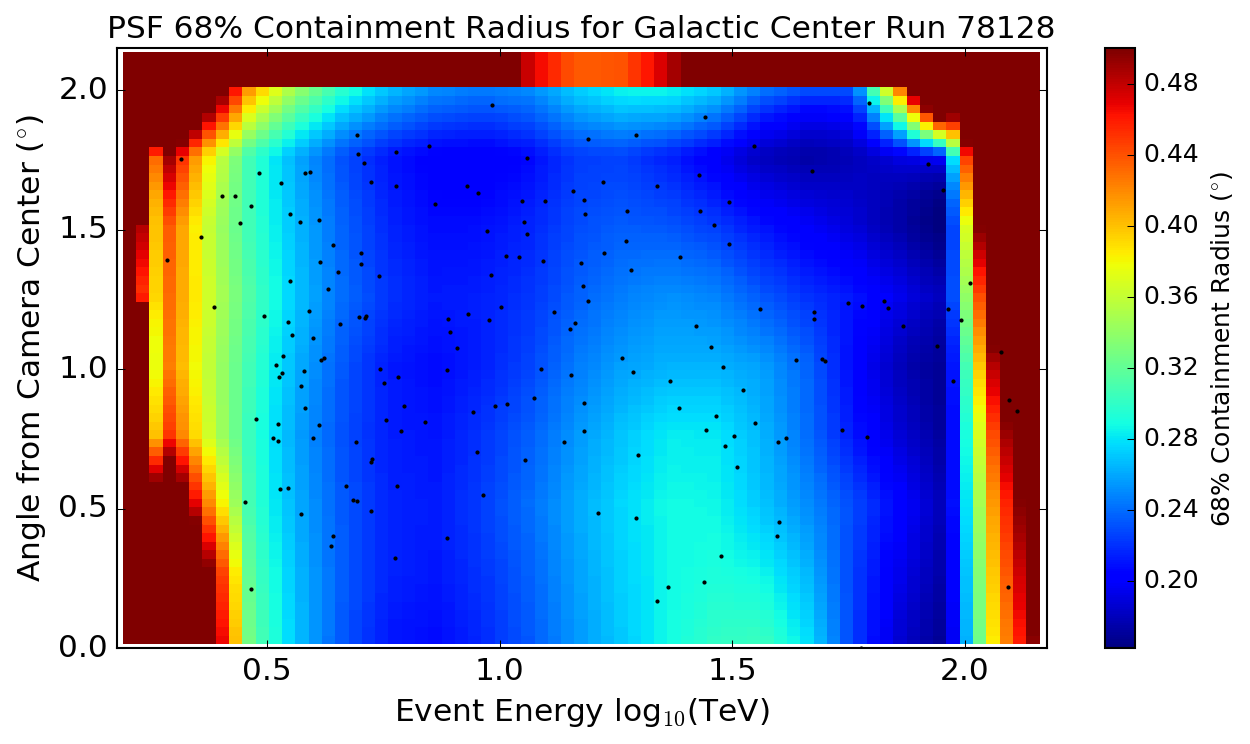
\includegraphics[width=0.95\textwidth]{images/psf_king_plots/psf_parameter_space.pdf}
      \caption[PSF Parameter Space]{
        The 68\% containment radius for the energy/offset parameter space for Sgr A* run 78128. 
        The black points are from data, showing a subset of the event locations from run 78128 in the parameter space.
        The color axis is the containment radius, calculated from simulations.
        While events from all energies are shown in this figure, only events from \SIrange{4}{70}{\TeV{}} are used in the analysis (see Section~\ref{sec:crab_analysis}).
      }
      \label{fig:psf_paramspace}
    \end{figure}

    For the Galactic Center and the Crab Nebula analyses, the distribution of 68\% containment radii for all events is shown in Figure~\ref{fig:gc_psf_hist}.
    The asymmetric structure is due to the varying effective area at different offsets and energies, which changes the distribution of events in the PSF table.
    The long tails are likely due to events at the edge of the observable energy and offset ranges, where the PSF gets worse.

    \begin{figure}[!hb]
      \centering
      \begin{tabular}{c}
        \includegraphics[width=0.85\textwidth]{images/psf_gc_eventhist/eventpsf_crab.pdf} \\
        \includegraphics[width=0.85\textwidth]{images/psf_gc_eventhist/eventpsf_sgra.pdf}
      \end{tabular}
      %\includegraphics[width=0.85\textwidth]{images/psf_gc_eventhist/eventpsf.pdf}
      \caption[Crab and Galactic Center Event PSFs]{
        The 68\% containment radius for all Crab Nebula and Sgr A* events used in this analysis.
      }
      \label{fig:gc_psf_hist}
    \end{figure}
  
  \FloatBarrier
  
  \subsection{Background Models}\label{background_production}
  
    A background model is a three-dimensional function in camera $x$ (a horizontal angle, parallel to azimuth), camera $y$ (a vertical angle, parallel to elevation), and energy.
    Each background model is constructed from one of two templates, and the templates are built from dark run observations (see Figure~\ref{fig:gcfieldsofview}).
    These background models calculate the number of expected events in the camera, per unit solid angle, unit time, and unit energy.
    This is used to quantify how many counts are expected in different parts of the camera when observing any target.
    Understanding the background shape of the camera is crucial for properly studying extended sources, like dark matter halos, which may extend several degrees from the Galactic Center.
    Improperly estimating background models can result in fake structures appearing around an astrophysical target.
    
    The background models used in this analysis are made from two background templates, one for each of the V5/V6 epochs (see Section~\ref{sec:epochs}).
    The templates are constructed from dark observations, detailed later in \ref{veritasdata}.
    Each template is made by binning all background events radially by camera position and by their energy, to produce a spectral function.
    This spectral function can be seen in Figure~\ref{fig:background_profile}.
    The radial function at two different energies is shown in Figure~\ref{fig:background_radial}.

    \begin{figure}[p]
      \centering
      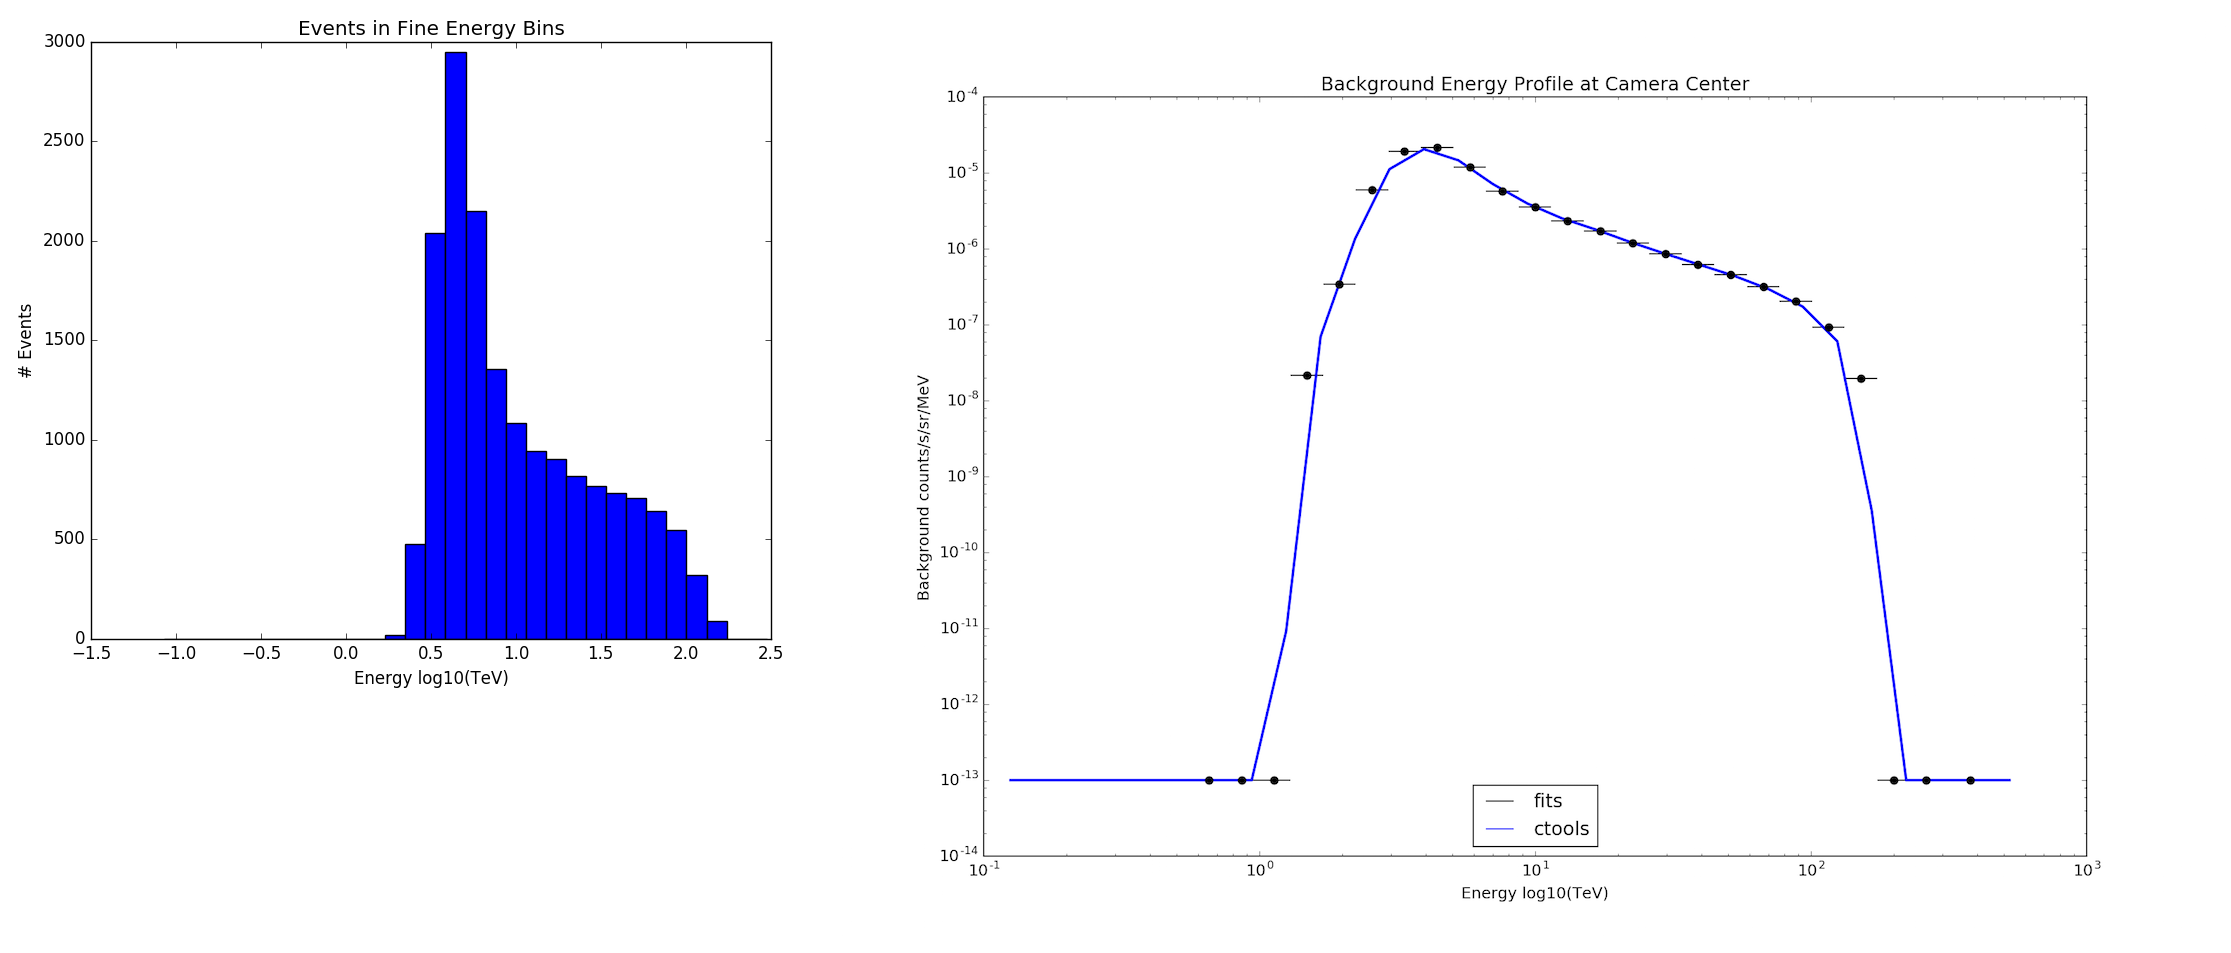
\includegraphics[width=0.6\textwidth]{images/ctools_background/background_construction.eps}
      \caption[CTOOLS Background Fine Energy Bins]{
        The V5 background's fine energy bins.
        The top plot shows the number of events in each energy bin from all background runs.
        The bottom plot shows the background rate, the number of background events divided by the observation time, solid angle, and energy span.
        The black points show the background rate in each energy bin, while the blue line shows the interpolated background rate.
      }
      \label{fig:background_profile}
    \end{figure}

    \begin{figure}[hb]
      \centering
      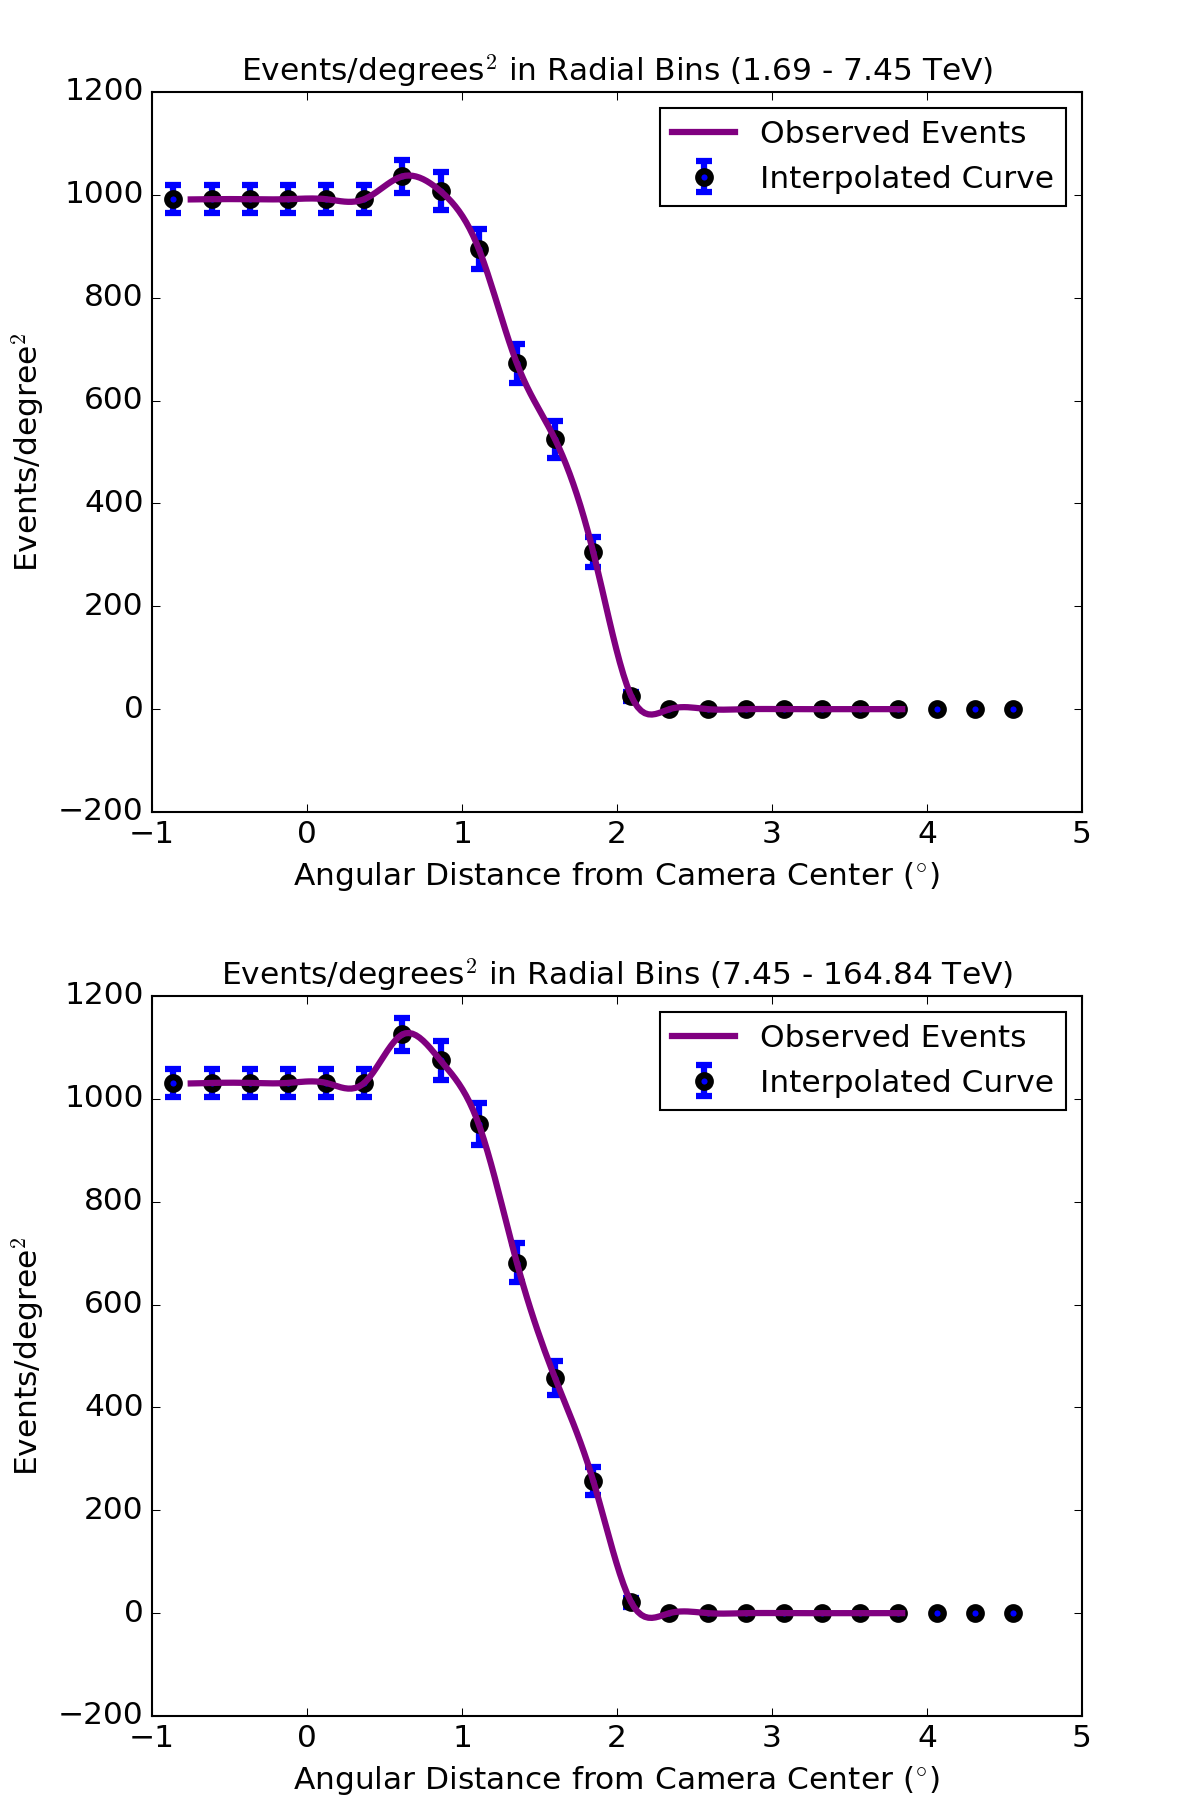
\includegraphics[width=0.5\textwidth]{images/ctools_background/radial_profiles.eps}
      \caption[CTOOLS Radial Background Profiles]{
        Radial bin profiles for the V5 backgrounds for low and high energies, to show how the shape varies with energy.
        The blue points are the counts per bin area, while the purple line is a spline interpolation with a 3rd order polynomial.
        The peak and plateau at \ang{0}-\ang{1} is due to the background events not being radially symmetric in the camera, due to the changing atmospheric depth across the camera's field of view.
        For fitting the interpolated curve, the bin values at angles less than \ang{0} are copied from the \ang{0} bin.
        The same is done for bins beyond \ang{2.5}, which are copies of the \ang{2.5} bin value.
        }
      \label{fig:background_radial}
    \end{figure}
    
    Finally, the spatial and spectral functions $M_{s} \left ( e \right )$ and $M_e \left(x,y,e \right )$ are multiplied together, as in
    
    \begin{equation}\label{eqn:bck_template}
      f(e,x,y) = A \, \times \, M_{e} \left ( e \right ) \, \times \, M_{s} \left ( x, y, e \right ) \,.
    \end{equation} 
    
    The function $f(e,x,a)$ has units of $\frac{\textrm{Number of Counts}}{ \textrm{MeV} \times \textrm{s} \times \textrm{sr} }$.
    The function $M_{e}(e)$ is a spectral function power law.
    The function $M_{s}(x,y,e)$ is a spatial template that varies with camera $x$, camera $y$, and energy $e$, built from Sgr A* Off data described in Section~\ref{veritasdata}.
    The multiplied functions are then scaled with a constant $A$ such that the total integral of the template (integrating across camera $x$, camera $y$, and energy) is equal to the original number of counts in the Sgr A* Off runs, as in
    
    \begin{equation}\label{eqn:background_template_function}
      \textrm{Number of Background Events} = A \, \int \, M_{e} \left ( e \right ) \, \times \, M_{s} \left ( x, y, e \right ) \; dx \: dy \: de \,.
    \end{equation}

    This function $f(e,x,y)$ is the background template in camera $x$ and $y$.
    Each background template is used in the likelihood analysis as a model multiplied by two free parameters, a normalization factor, and the event energy exponentiated by the spectral index.
    This lets the likelihood fitter scale each run's background model up or down to best match the number of observed events.
    This means the analysis is less dependent on the background's absolute value, and more dependent on the relative values in different parts of the camera background or at different energies.
  
  \FloatBarrier

  \subsection{Energy Dispersion}\label{subsec:edisp}
    As events are reconstructed imperfectly, it is important to understand what the distribution of reconstructed energies are for a given true energy.
    This \textit{dispersion in energy} is quantified by an energy migration matrix $E_{i,j}$, where $i$ denotes the $i^{\text{th}}$ reconstructed energy bin, and $j$ denotes the $j^{\text{th}}$ true energy bin.
    A migration matrix is created by simulating many showers at a variety of true energies and binning them based on their true and reconstructed energies.
    Several matrices are then created, by grouping showers into bins based on their distance from the camera center.
    
    Because simulations are computationally expensive, only a limited number can be produced for each migration matrix.
    At some places in the matrix, low simulation statistics can artificially alter the shape of the matrix.
    To reduce the effect of this, interpolation is applied to the matrix.
    The number of events at a particular place in the matrix is then found by interpolating from neighboring true energy, reconstructed energy, and angular offset bins in this table.
    This interpolated  energy migration matrix can be used to account for two significant effects.
    
    The first is that the reconstruction method introduces biases in the event energy, meaning an event at a given true energy can be reconstructed on average at a higher or lower energy.
    The second effect that is accounted for is the dispersion in the reconstructed energies.
    Gamma rays with the same energy will have their energies reconstructed as a distribution close to the true energy.
    These fluctuations can be due to randomness in air shower development or atmospheric absorption of Cherenkov photons.
    This has the effect of distributing events in each energy bin of a spectra.
    In the gamma-ray spectra of astrophysical sources, which often follow a power law, lower energy bins tend to have more events than higher energy bins.
    This results in lower-energy dispersion contributing more to the higher-energy bins than the higher-energy dispersion contributes to the lower-energy bins.
    When not accounted for, this energy dispersion will harden observed astrophysical spectra.
    
    In Figure~\ref{fig:migmatrix}, an interpolated migration matrix is shown.
    Events at a given \ETrue{} are reconstructed at a spread of \EReco{}.
    This spread is due to the variability in how air showers develop in the atmosphere.
    Small variations early in the shower can have a large impact on the shower's Cherenkov image, meaning the shower can appear as though it was from a higher- or lower-energy gamma ray.
    At the lowest \ETrue{} energies some showers fluctuate upwards to produce more Cherenkov light, and consequently get reconstructed to higher \EReco{} energies.
    At the highest \ETrue{} energies, showers may be so large that they fill the entire camera, leading to lost photons past the edge of the camera, which cause the shower's energy to be reconstructed lower than it actually is.

    \begin{figure}[!th]
      \centering
      \includegraphics[width=0.85\textwidth]{images/edisp_plots/edisp.pdf}
      \caption[Energy Migration Matrix]{
        An energy migration matrix used with Sgr A* run 82288.
        The reconstructed energy is on the x-axis, and the true energy is on the y-axis.
        The z (color) axis denotes the interpolated number of simulated events that passed all cuts (see text for details).
        The dark-blue region from \SIrange{4}{70}{TeV} \EReco{} is the range of energies used in this analysis.
      }
      \label{fig:migmatrix}
    \end{figure}
  
  \FloatBarrier

\section{Camera Studies}
The objective of this thesis is to search for dark matter via the existence of a gamma-ray halo that is both extended and faint.
The extension and faintness of the halo, plus the relatively large amount of noise near the Galactic Center, prioritize understanding how the VERITAS camera behaves in high-noise conditions.
In order to better understand the camera's behavior in the reconstruction method, several studies were performed.

\subsection{Background Structure at the Low Energy Threshold}\label{subsec:bkgstructure}
To produce background models, events were binned according to their energy, telescope pointing elevation, and elevation and azimuth about the camera center.
As a result of this detailed binning, some new effects were noted.
First, Sgr A* Off data was reconstructed, which has no known gamma-ray source in its field of view.
The time spent at each telescope elevation is shown in Figure~\ref{fig:back_elevhist}.
To reduce the effect of the varying telescope elevation, time cuts were applied to select data between \ang{28.5} and \ang{29.5} telescope elevations.
This was done to reduce any effects of a large range of telescope elevations.
Because the shape of the atmospheric interaction volume strongly depends on the telescope elevation, a small elevation range helps isolate atmosphere-dependent effects.
Note that this is a cut on the telescope pointing, not on the actual event elevations.

\begin{figure}[bt]
  \centering
  \includegraphics[width=0.6\textwidth]{images/background_gradient_replot/sgraoff_1_hist_elev.pdf}
  \caption[Elevation Slice of Sgr A* Off Data]{
    Time spent pointing the observatory at each elevation.
    Blue is all Sgr A* Off data, while green is the selected pointing elevations used in Figure~\ref{fig:background_grid}.
  }
  \label{fig:back_elevhist}
\end{figure}
    
Gamma-like events were then selected from this data, and binned in energy in Figure~\ref{fig:background_grid}.
The left histograms show the number of events at each energy.
For each row, a different energy range is selected, shown in green in the left plot.
The cuts to pointing-elevation and energy are applied, and the surviving events are then histogrammed in the right-hand plots according to their azimuth and elevation in the camera.
    
As a measure of how far the events deviate from the camera center, an orange dot and circle are also plotted.
These indicate the average event position, and the 68\% containment radius around that position.
Figure~\ref{fig:background_grid} shows that at the lowest energies, events are reconstructed and pass cuts only in the top half of the camera.
This is because at this low \ang{29} elevation, the atmospheric column density is \nicetilde13\% lower at the top of the camera than at the bottom.
% see veripy.atmo_column_density()
This allows lower-energy gamma rays and their showers' Cherenkov photons to get closer to the observatory, making them easier to detect.
Below this energy, gamma rays do not produce enough Cherenkov photons to survive past the atmospheric scattering and PMT quantum efficiency.
The bottom of the camera has more atmosphere, however, and can be considered opaque to gamma rays \SI{2.5}{TeV} and lower.
At higher energies a similar effect is also noted, where the events cluster in the bottom half of the camera more than the top half.
As atmospheric column density is higher in that part of the camera, higher energy showers may be created farther away, where the observatory's fixed-angle opening views a much larger volume of the atmosphere, detecting more showers.

\begin{figure}[p]
  \centering
  \begin{tabular}{rl}
    \newcommand{\lwidth}{6.5}
    \newcommand{\rwidth}{4}
    \subfloat{\includegraphics[width=5.5cm]{images/background_gradient_replot/sgraoff_1_hist_energy.pdf}} & 
    \subfloat{\includegraphics[width=3.0cm]{images/background_gradient_replot/sgraoff_1_cam.pdf}}         \\
    \subfloat{\includegraphics[width=5.5cm]{images/background_gradient_replot/sgraoff_2_hist_energy.pdf}} & 
    \subfloat{\includegraphics[width=3.0cm]{images/background_gradient_replot/sgraoff_2_cam.pdf}}         \\
    \subfloat{\includegraphics[width=5.5cm]{images/background_gradient_replot/sgraoff_3_hist_energy.pdf}} & 
    \subfloat{\includegraphics[width=3.0cm]{images/background_gradient_replot/sgraoff_3_cam.pdf}}         \\
    %\subfloat{\includegraphics[width=7.5cm]{images/background_gradient_replot/sgraoff_4_hist_energy.pdf}} & 
    %\subfloat{\includegraphics[width=4.5cm]{images/background_gradient_replot/sgraoff_4_cam.pdf}} 
    \subfloat{\includegraphics[width=5.5cm]{images/background_gradient_replot/sgraoff_5_hist_energy.pdf}} & 
    \subfloat{\includegraphics[width=3.0cm]{images/background_gradient_replot/sgraoff_5_cam.pdf}}         \\
    \subfloat{\includegraphics[width=5.5cm]{images/background_gradient_replot/sgraoff_6_hist_energy.pdf}} & 
    \subfloat{\includegraphics[width=3.0cm]{images/background_gradient_replot/sgraoff_6_cam.pdf}}         \\
    \subfloat{\includegraphics[width=5.5cm]{images/background_gradient_replot/sgraoff_7_hist_energy.pdf}} & 
    \subfloat{\includegraphics[width=3.0cm]{images/background_gradient_replot/sgraoff_7_cam.pdf}} 
  \end{tabular}
  \caption[Atmospheric Gradient in the VERITAS Camera]{
    Event energies and camera backgrounds after the pointing elevation cut shown in Figure~\ref{fig:back_elevhist}.
    In the left histograms, blue is all events while green is events in the selected energy range.
    The right shows 2D histograms, made from the camera azimuths and elevations using the green events selected in the histogram to its left.
    The orange dot and circle denote the average event position, and 68\% containment radius for the events in the plot.
    The \SIrange{1.8}{3.2}{TeV} energy range shows events are detected more in the upper half of the camera.
    From \SIrange{4}{6}{TeV}, events are more in the bottom half of the camera, while from \SIrange{6}{70}{TeV} events are closer to the camera center.
  }
  \label{fig:background_grid}
\end{figure}
    
These effects are visible in the galactic ($l$,$b$) event maps from data.
In Figure~\ref{fig:bkgvsel_crab}, the top plot shows the positions of all events from several hours of Crab Nebula data.
The location of the Crab Nebula is marked in blue, while the red circle and point indicate the average event position and radius containing 68\% of the events.
The middle histogram shows the distribution of event energies, and the bottom plot shows the positions of events in a limited energy range, \SIrange{1.5}{3.25}{\TeV{}}.
The middle plot indicates a specific energy range used in the bottom plot.
When events in this limited energy range are plotted in the bottom plot, the average event position (the red dot) shifts upwards by \ang{0.32}.
This is due to fewer events appearing in the bottom of the camera, due to the thicker atmosphere there.
    
% plots produced by $V/thesis/plots/background_vs_elevation/background_vs_elevation.py
% filters events between telescope pointing elevations 28.5 and 29.5
% 
% text output from background_vs_elevations.py :
% Crab, 165 fits
% 26766 raw events
% 2400 elev events
% Crab at: lb: 184.5576 -5.7842 deg
% Crab 1.0-200.0TeV avg lb: 184.5865 -5.7486 deg  frac=0.6827 containment radius:1.4210
% Crab 1.5-3.2TeV   avg lb: 184.6435 -5.4282 deg  frac=0.6827 containment radius:1.3104
%
% Sgr A*, 969 fits
% 160924 raw events
% 90896 elev events
% Sgr A* at:  lb: 359.9442 -0.0460 deg
% Sgr A* 1.0-200.0TeV avg lb: 359.9102 -0.0584 deg  frac=0.6827 containment radius:1.4710
% Sgr A* 1.5-3.2TeV   avg lb: 0.2546    0.1457 deg  frac=0.6827 containment radius:1.4139
\begin{figure}[p]
  \centering
  %\includegraphics[height=0.85\textheight]{images/background_vs_elevation/background_vs_elevation_srccrab.eps}
  \includegraphics[height=0.85\textheight]{images/background_vs_elevation/background_vs_elevation_crab.pdf}
  \caption[Background Vs Elevation Crab Nebula]
  {\small 
    Plots of Crab Nebula observations.
    Top: Sky map of all events.
    Middle: Histogram of all events in energy.
    Bottom: Sky map of events from \SIrange{1.5}{3.25}{\TeV{}}.  
    Data is first filtered so that the telescope pointing is between elevations of \ang{28.5} and \ang{29.5}.
    Red dots and circles are the average event positions and the 68\% containment radii.
  }
  \label{fig:bkgvsel_crab}
\end{figure}
    
\begin{figure}[p]
  \centering
  %\includegraphics[height=0.85\textheight]{images/background_vs_elevation/background_vs_elevation_srcsgra.eps}
  \includegraphics[height=0.85\textheight]{images/background_vs_elevation/background_vs_elevation_sgra.pdf}
  \caption[Background Vs Elevation Sgr A*]
  {\small 
    Plots of Sgr A* observations.
    Top: Sky map of all events.
    Middle: Histogram of all event energies.
    Bottom: Sky map of events from \SIrange{1.5}{3.25}{\TeV{}}.  
    Data is first filtered so that the telescope pointing is between elevations of \ang{28.5} and \ang{29.5}.
    Red dots and circles are the average event positions and the 68\% containment radii.
  }
  \label{fig:bkgvsel_sgra}
\end{figure}

When similar plots are made for the Galactic Center in Figure~\ref{fig:bkgvsel_sgra}, the effect is much stronger, and rotated.
In the top plot, events are radially symmetric around the source position.
The red dot and circle are the average event position and the 68\% containment radius.
When only the events from \SIrange{1.5}{3.25}{\TeV{}} are plotted, the average event position moves by \ang{0.4}, due to a deficit in the lower right part of the plot.
This area corresponds to the bottom of the low-energy camera plots in Figure \ref{fig:background_grid}.
The rotation occurs when converting between camera x/y coordinates (Earth Elevation/Azimuth) and Galactic coordinates ($l$,$b$).
The degree of rotation also changes from run to run, which further blurs this effect.
For the Crab Nebula plots in Figure~\ref{fig:bkgvsel_crab}, the rotation is only a few degrees, while for Sgr A* in Figure~\ref{fig:bkgvsel_sgra}, it is closer to \ang{70}.
    
This effect is important to the analysis because it implies that, at the lowest energies, the background rate is not radially symmetric.
Radial backgrounds (sometimes referred to as acceptances) are typically used in VERITAS, as no other camera $x$/$y$ or energy dependence had been demonstrated until now.
Due to a limited amount of background data (see Table~\ref{tab:observation_times}), only radially-dependent backgrounds are used in this analysis.
To attempt to reduce the effect of the non-uniform atmosphere, the event energies were limited to \SIrange{4}{70}{TeV}.
Even with this limited energy range, the atmospheric effect is still prominent, and studied further in Section~\ref{sec:elevgradient}.

Additional studies were performed to test if bright stars near the Galactic Center might affect a dark matter search, and are detailed in Appendix~\ref{app:starpixels}.
Bright stars were found to have a negligible effect, and were ignored in this analysis.

\FloatBarrier

